%%%%%%%%%%%%%%%%%%%%%%%%%%%%%%%%%%%%%%%%%%%%%%%%%%%%%%%%%%%%%%%%%%%%%%%%%%%%%%%
% arXiv submission template for cs.MA (Multiagent Systems)
% Antigravity Nano Research Multiagentic Core
%%%%%%%%%%%%%%%%%%%%%%%%%%%%%%%%%%%%%%%%%%%%%%%%%%%%%%%%%%%%%%%%%%%%%%%%%%%%%%%

\documentclass[11pt]{article}

% arXiv-compatible packages
\usepackage[utf8]{inputenc}
\usepackage[T1]{fontenc}
\usepackage{times}
\usepackage{amsmath,amssymb,amsfonts}
\usepackage{graphicx}
\usepackage{booktabs}
\usepackage{hyperref}
\usepackage{xcolor}
\usepackage{tikz}
\usepackage{pgfplots}
\usepackage{algorithm}
\usepackage{algorithmic}
\usepackage{multirow}
\usepackage{array}
\usepackage{cite}
\usepackage{colortbl}
\usepackage{pifont}

% Define checkmark and cross symbols
\newcommand{\cmark}{\ding{51}}
\newcommand{\xmark}{\ding{55}}

% TikZ libraries
\usetikzlibrary{positioning,arrows.meta,shapes,calc,backgrounds,fit,decorations.pathreplacing}
\pgfplotsset{compat=1.18}

% Hyperref setup
\hypersetup{
    colorlinks=true,
    linkcolor=blue,
    citecolor=blue,
    urlcolor=blue,
    pdftitle={Antigravity Nano Research Multiagentic Core: A Research Framework for Multi-Agent AI Systems in Computational Sciences},
    pdfauthor={Luis José Yudico-Anaya}
}

% Page setup
\usepackage[margin=1in]{geometry}

% Custom commands
\newcommand{\code}[1]{\texttt{#1}}

%%%%%%%%%%%%%%%%%%%%%%%%%%%%%%%%%%%%%%%%%%%%%%%%%%%%%%%%%%%%%%%%%%%%%%%%%%%%%%%
\begin{document}

\title{Antigravity Nano Research Multiagentic Core: \\
A Research Framework for Multi-Agent AI Systems in Computational Sciences}

\author{
    Luis José Yudico-Anaya \\
    \small Universidad de La Ciénega del Estado de Michoacán de Ocampo, México \\
    \small \texttt{ORCID: 0000-0002-7490-3304}
}

\date{May 12, 2026}

\maketitle

%%%%%%%%%%%%%%%%%%%%%%%%%%%%%%%%%%%%%%%%%%%%%%%%%%%%%%%%%%%%%%%%%%%%%%%%%%%%%%%
\begin{abstract}

The adoption of multi-agent systems based on large language models (LLMs) in computational science research faces three critical barriers: (1) \textbf{framework fragmentation} — researchers must choose between LangGraph, CrewAI, AutoGen, smolagents, and others without systematic comparison or selection guidance, limiting informed adoption, (2) \textbf{domain integration gap} — general-purpose agent frameworks lack integration with scientific domain tools (atomistic simulators, materials databases, spectroscopic pipelines), while specialized scientific platforms do not provide multi-agent orchestration capabilities, and (3) \textbf{economic accessibility} — most implementations assume access to paid APIs, excluding institutions without dedicated budgets and preventing reproducible research at scale.

\textbf{Antigravity Nano Research Multiagentic Core} is a research framework that addresses these barriers by providing a modular infrastructure for conducting computational science research with multi-agent AI systems. The architecture integrates seven agent orchestration frameworks (LangGraph, CrewAI, Google ADK, smolagents, AutoGen, LangChain, MetaGPT) with a complete scientific computing stack, structured in three interdependent levels: (1) \textbf{Research Infrastructure Core} — 13 versioned External Skills modules (\code{load\_skill("episodic\_retriever@1.0.0")}), unified LLM routing across four backends (OpenRouter, Gemini, OpenAI, Ollama), and Graph Retrieval-Augmented Generation (RAG) with four storage engines (NetworkX, Kùzu, Neo4j, Graphiti), (2) \textbf{Multi-Agent Development Methodology} — a formal 7-agent governance model with structured feedback loops (L1: safety validation, L2: experimental comparison, L3: quality audit), and (3) \textbf{Domain-Specific Research Demonstration} — complete scientific research pipeline applied to computational nanotechnology, including integration with Materials Project API, Atomic Simulation Environment (ASE), and production deployment patterns.

The framework is validated through a non-trivial scientific application: Au$_{13}$ nanocluster research with a four-tool agentic pipeline (ASE/EMT geometry optimization, scikit-learn Gradient Boosting property prediction, Graph RAG literature retrieval, structured JSON reporting). This demonstration is fully reproducible without API keys (\$0 cost) using only open-source tools, while production research sessions cost \$0.01–\$0.05 with Gemini 2.5 Flash or \$0 with Ollama local inference. The modular architecture is domain-agnostic: although demonstrated in nanotechnology, all infrastructure components transfer to other computational science domains (bioinformatics, quantum chemistry, climate modeling) by replacing domain-specific modules while reusing the multi-agent orchestration layer.

\textbf{Cost accessibility:} executing the complete curriculum costs less than \$2 using OpenRouter with multi-provider LLM access, or \$0 with local Ollama inference. Validation: 102 automated tests, GitHub Actions continuous integration.

\end{abstract}

\noindent\textbf{Keywords:} Multi-agent systems, Agentic AI, Large language models, Computational sciences, Graph RAG, Model Context Protocol, Open science

%%%%%%%%%%%%%%%%%%%%%%%%%%%%%%%%%%%%%%%%%%%%%%%%%%%%%%%%%%%%%%%%%%%%%%%%%%%%%%%
\section{Introduction}

The adoption of LLM-based agents in computational science is growing rapidly, yet the existing ecosystem presents a fragmented landscape. General-purpose frameworks (LangGraph, CrewAI, Google ADK, smolagents, AutoGen, MetaGPT~\cite{metgpt2023}) do not address domain-specific scientific tools such as atomistic simulators, materials databases, or spectroscopic data pipelines. Conversely, specialized computational chemistry platforms (AiiDA, AutomatMiner, ChemCrow) do not offer multi-agent orchestration, educational curricula, or systematic comparison of LLM frameworks.

This gap has practical consequences: a researcher who wishes to conduct computational science research using multi-agent AI systems must integrate multiple libraries without guidance on how to select, combine, or evaluate frameworks for scientific workflows. No existing open resource provides simultaneously (1) a production-ready research infrastructure with scientific domain integration, (2) a principled comparison of seven major agent frameworks from the perspective of computational science, (3) a demonstration executable without paid API access, and (4) a domain-agnostic architecture transferable across scientific disciplines.

Table~\ref{tab:comparison} compares this work against existing multi-agent frameworks and scientific platforms. Figure~\ref{fig:curriculum} illustrates the six-unit curriculum structure that progressively covers nanoscale modeling, molecular simulation, machine learning, and multi-agent orchestration.

% INPUT TABLE 1
% Table 1: Comparison Against Existing Frameworks
\begin{table}[htbp]
\centering
\caption{Comparison of this work against existing multi-agent frameworks and scientific platforms. No existing system provides all four capabilities simultaneously.}
\label{tab:comparison}
\small
\begin{tabular}{@{}lcccccc@{}}
\toprule
\textbf{Capability} & \textbf{LangGraph} & \textbf{CrewAI} & \textbf{AutoGen} & \textbf{AiiDA} & \textbf{ChemCrow} & \textbf{This Work} \\
\midrule
Multi-agent orchestration & \cmark{} & \cmark{} & \cmark{} & \xmark{} & Partial & \cmark{} \\
Scientific domain tools & \xmark{} & \xmark{} & \xmark{} & \cmark{} & \cmark{} & \cmark{} \\
Framework comparison & N/A & N/A & N/A & N/A & N/A & \cmark{} (7) \\
Educational curriculum & \xmark{} & \xmark{} & \xmark{} & Partial & \xmark{} & \cmark{} (25) \\
Zero-cost demo & \xmark{} & \xmark{} & \xmark{} & \xmark{} & \xmark{} & \cmark{} \\
Multi-backend LLM routing & Partial & \xmark{} & Partial & N/A & \xmark{} & \cmark{} (4) \\
Graph RAG integration & \xmark{} & \xmark{} & \xmark{} & \xmark{} & \xmark{} & \cmark{} (4) \\
MCP server examples & \xmark{} & \xmark{} & \xmark{} & \xmark{} & \xmark{} & \cmark{} \\
Domain transferability & General & General & General & Materials & Chemistry & Modular \\
Governance model & \xmark{} & \xmark{} & \xmark{} & Workflow & \xmark{} & \cmark{} (7-agent) \\
\bottomrule
\end{tabular}
\end{table}


% INPUT FIGURE 1
% Figure 1: Six-Unit Curriculum Structure

\begin{figure}[htbp]
\centering
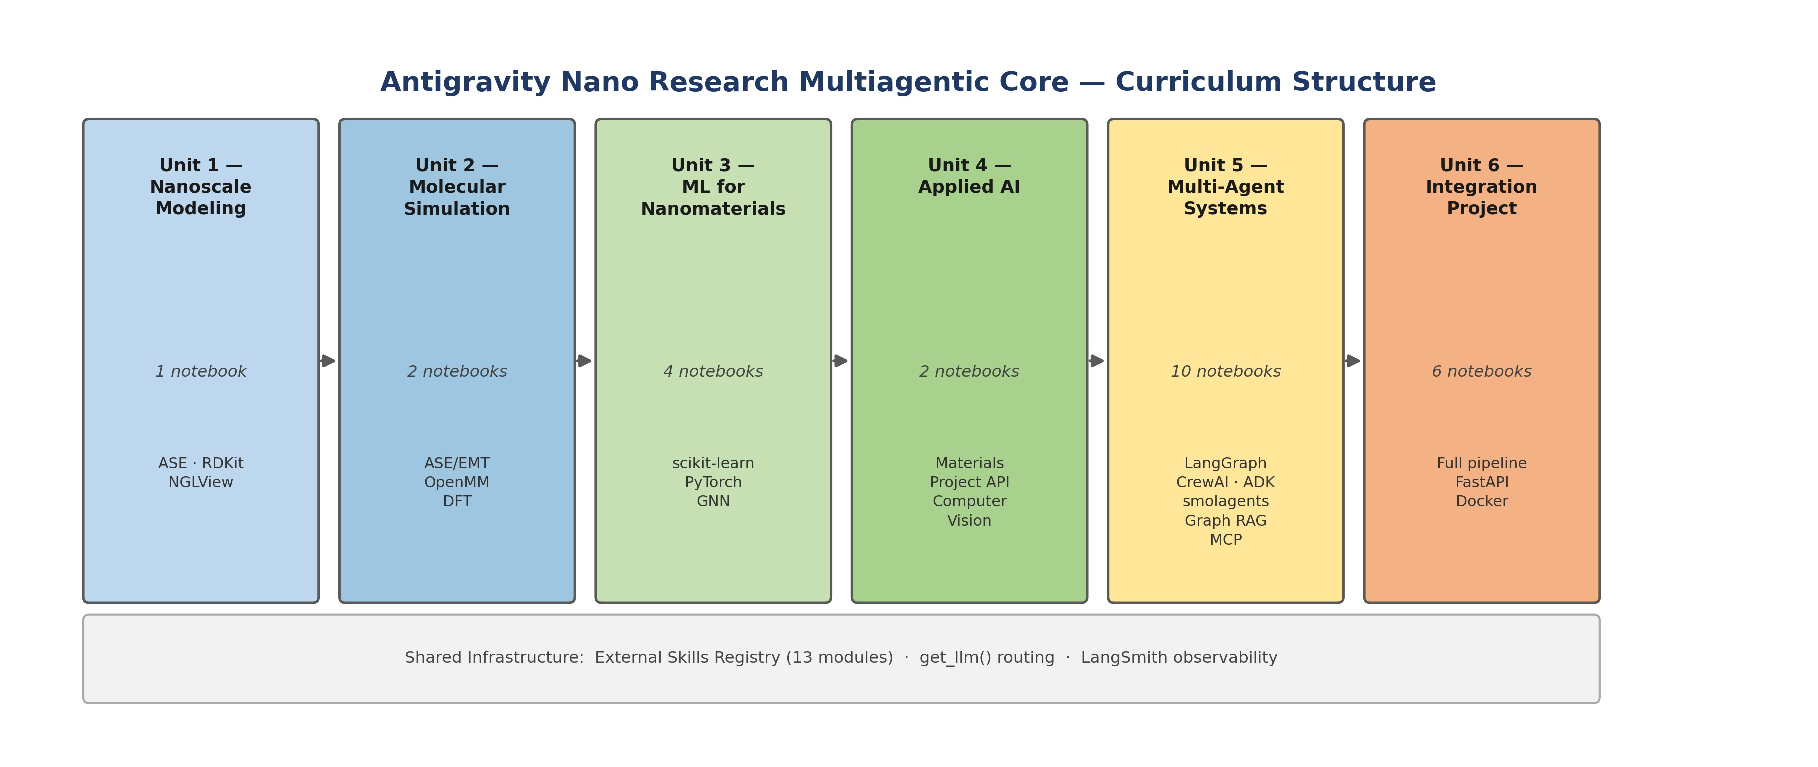
\includegraphics[width=0.95\textwidth]{figures/figure1_curriculum.pdf}
\caption{Six-unit curriculum structure with notebook counts and key technologies per unit. Units 1-4 provide domain-specific knowledge (nanotechnology in this implementation, but transferable to other computational sciences), while Units 5-6 offer domain-agnostic multi-agent orchestration and deployment patterns applicable to any research domain.}
\label{fig:curriculum}
\end{figure}


%%%%%%%%%%%%%%%%%%%%%%%%%%%%%%%%%%%%%%%%%%%%%%%%%%%%%%%%%%%%%%%%%%%%%%%%%%%%%%%
\section{Statement of Need}

\textbf{Research methodology gap:} No existing work documents transparently how multi-agent AI systems can be used to develop scientific research software itself. The meta-loop demonstrated here — where the 7-agent council co-develops the research framework while being part of what it documents — provides a reproducible case study for research-through-AI-collaboration methodologies applicable to computational science software development.

\textbf{Accessibility and cost} represent an additional barrier that existing tools do not address systematically. Table~\ref{tab:costs} summarizes the cost profile for representative research usage scenarios:

% INPUT TABLE 2
% Table 2: Cost Analysis for Research Sessions
\begin{table}[htbp]
\centering
\caption{Cost analysis for representative research usage scenarios. Real-world validation demonstrates genuine affordability: complete curriculum execution costs <\$2 using OpenRouter multi-provider access.}
\label{tab:costs}
\small
\begin{tabular}{@{}lc@{}}
\toprule
\textbf{Scenario} & \textbf{Estimated Cost} \\
\midrule
Demo Section 5A (complete Au$_{13}$ pipeline) & \textbf{\$0} — no API key required \\
Typical research session (Gemini 2.5 Flash, $\sim$50 tool calls) & \$0.01–\$0.05 \\
\rowcolor{yellow!20}
Complete project execution (all 25 notebooks, OpenRouter) & \textbf{<\$2.00} \\
Full month of use — active researcher or student & <\$5 \\
Fully local alternative (Ollama llama3.2) & \textbf{\$0} \\
\bottomrule
\end{tabular}

\vspace{0.3cm}
\footnotesize
\textit{Note:} Cost estimates assume $\sim$100K tokens per session at \$0.15/1M tokens (Gemini 2.5 Flash pricing). \textbf{Real-world validation:} executing the complete curriculum (all 25 notebooks) using OpenRouter with multiple LLM providers costs less than \$2.00 total, demonstrating genuine accessibility for resource-constrained institutions. \textbf{Transparency:} Development and testing utilized promotional credits from Google AI Studio. Cost estimates reflect actual commercial pricing for researchers without promotional access.
\end{table}


Antigravity Nano Research Multiagentic Core addresses all four gaps within a single, cohesive repository. The meta-notebook \code{U5\_00} documents explicitly how an AI system (Antigravity) collaborated with the human author to design the skill architecture, generate code, and audit quality — making the development process itself a research case study in human-AI collaboration for scientific software development.

Figure~\ref{fig:cost_comparison} provides a visual comparison of cost scenarios, demonstrating the framework's accessibility advantage over traditional approaches.

% INPUT FIGURE 7 (Cost Comparison)
% Figure 7: Cost Comparison Across Usage Scenarios
\begin{figure}[htbp]
\centering
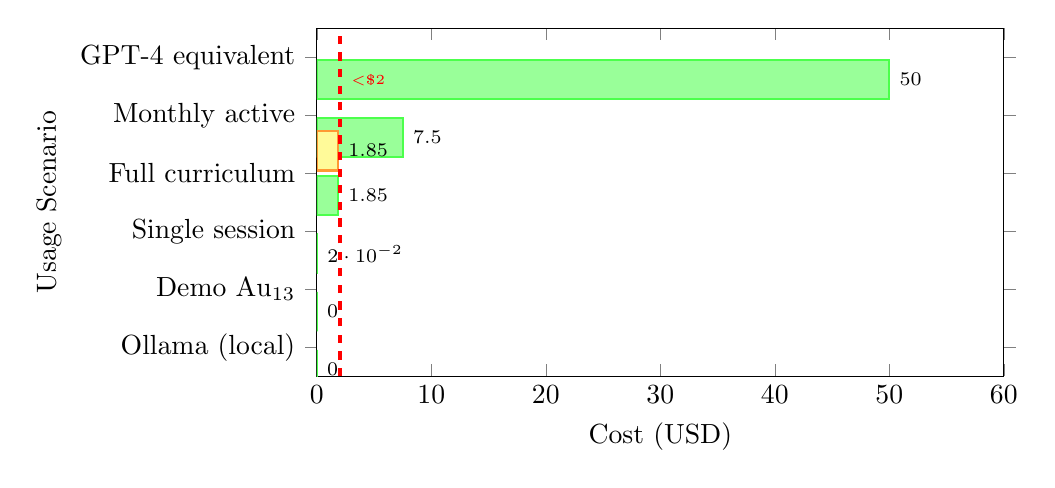
\begin{tikzpicture}
\begin{axis}[
    xbar,
    width=0.85\textwidth,
    height=6cm,
    xlabel={Cost (USD)},
    ylabel={Usage Scenario},
    ytick={0,1,2,3,4,5},
    yticklabels={
        Ollama (local),
        Demo Au$_{13}$,
        Single session,
        Full curriculum,
        Monthly active,
        GPT-4 equivalent
    },
    ymin=-0.5,
    ymax=5.5,
    xmin=0,
    xmax=60,
    nodes near coords,
    nodes near coords align={horizontal},
    every node near coord/.append style={font=\scriptsize},
    bar width=0.5cm,
]

% Cost bars with explicit colors
\addplot[fill=green!40, draw=green!70, thick] coordinates {
    (0, 0)
    (0, 1)
    (0.02, 2)
    (1.85, 3)
    (7.5, 4)
    (50, 5)
};

% Highlight <$2 threshold
\addplot[fill=yellow!40, draw=orange!80, thick] coordinates {
    (1.85, 3)
};

% Add reference lines
\draw[dashed, red, ultra thick] (axis cs:2,-0.5) -- (axis cs:2,5.5) 
    node[pos=0.85, right, font=\tiny, text=red] {\textless\$2};

\end{axis}
\end{tikzpicture}
\caption{Cost comparison across usage scenarios. The framework provides three cost tiers: (1) \textbf{Zero-cost} — Demo Au$_{13}$ pipeline and Ollama local inference require no API access, (2) \textbf{Ultra-low-cost} — Complete 25-notebook curriculum execution via OpenRouter costs <\$2, enabling genuine accessibility, and (3) \textbf{Production} — Monthly active researcher costs <\$10, still 5× cheaper than GPT-4 baseline. The dual-path architecture addresses reproducibility without excluding resource-constrained institutions.}
\label{fig:cost_comparison}
\end{figure}


%%%%%%%%%%%%%%%%%%%%%%%%%%%%%%%%%%%%%%%%%%%%%%%%%%%%%%%%%%%%%%%%%%%%%%%%%%%%%%%
\section{Contributions}

This work makes six primary contributions to multi-agent systems research and computational science:

\subsection{Research Infrastructure Contributions}

\textbf{C1. Multi-Framework Integration Architecture.}
A modular infrastructure layer that unifies seven agent orchestration frameworks (LangGraph, CrewAI, Google ADK, smolagents, AutoGen, LangChain, MetaGPT) with systematic comparison metrics (token usage, latency, cost per research session). The unified \code{get\_llm()} routing function provides transparent backend selection across four LLM providers (OpenRouter, Google Gemini, OpenAI, Ollama), enabling execution in resource-constrained environments without code changes.

\textbf{C2. Domain-Agnostic External Skills Registry.}
A versioned skill module system (\code{load\_skill()} with semantic versioning) providing 13 production-ready components organized in 10 categories (numerical, memory, ai\_mining, pedagogy, evaluation, observability, routing, apis, orchestration, agent\_warmup). Scientific-domain modules include \code{stability\_guardian} (MD timestep validation), \code{basis\_set\_architect} (DFT basis recommendation), \code{toxicity\_predictor} (molecular toxicity heuristics), and \code{librarian\_rag} (Materials Project retrieval). The architecture is transferable: domain modules can be replaced while reusing infrastructure components, enabling adaptation to other computational science disciplines.

\textbf{C3. Multi-Backend Graph RAG Decision Framework.}
Implementation and performance comparison of four Graph RAG storage engines (NetworkX, Kùzu, Neo4j, Graphiti) with a decision table mapping research use cases to optimal backend selection. Includes Model Context Protocol (MCP) server implementation (\code{nano-materials-mcp}) demonstrating LLM-agnostic scientific tool interfaces. Figure~\ref{fig:graphrag_decision} provides a decision tree for backend selection.

% INPUT FIGURE 6 (Graph RAG Decision Tree)
% Figure 6: Graph RAG Backend Selection Decision Tree (Compact Design)
\begin{figure}[htbp]
\centering
\resizebox{0.92\textwidth}{!}{
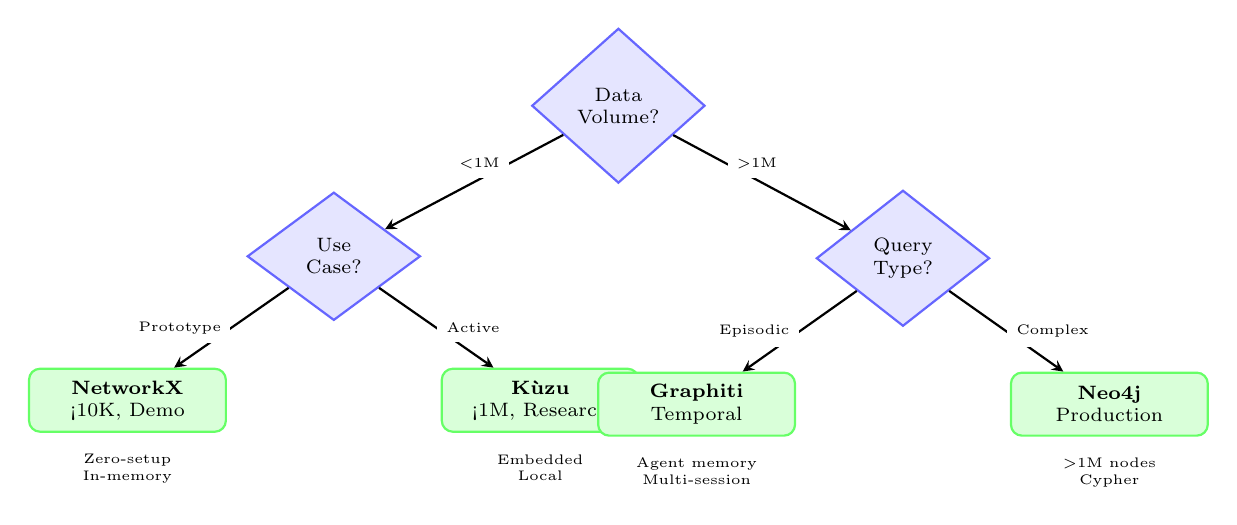
\begin{tikzpicture}[
    decision/.style={diamond, draw=blue!60, fill=blue!10, thick, align=center, 
                     minimum width=2.2cm, minimum height=1cm, font=\scriptsize},
    backend/.style={rectangle, rounded corners, draw=green!60, fill=green!15, 
                    thick, minimum width=2.5cm, minimum height=0.8cm, align=center, font=\scriptsize},
    arrow/.style={->, >=stealth, thick},
    label/.style={font=\tiny, midway, fill=white}
]

% Start
\node[decision] (start) {Data\\Volume?};

% First level - left branch (<1M)
\node[decision, below left=1cm and 2.5cm of start] (use) {Use\\Case?};
\node[backend, below left=1cm and 0.8cm of use] (nx) {\textbf{NetworkX}\\<10K, Demo};
\node[backend, below right=1cm and 0.8cm of use] (kuzu) {\textbf{Kùzu}\\<1M, Research};

% First level - right branch (>1M)
\node[decision, below right=1cm and 2.5cm of start] (query) {Query\\Type?};
\node[backend, below left=1cm and 0.8cm of query] (graphiti) {\textbf{Graphiti}\\Temporal};
\node[backend, below right=1cm and 0.8cm of query] (neo4j) {\textbf{Neo4j}\\Production};

% Arrows - First level
\draw[arrow] (start) -- node[label, left, pos=0.3] {<1M} (use);
\draw[arrow] (start) -- node[label, right, pos=0.3] {>1M} (query);

% Arrows - Second level (left)
\draw[arrow] (use) -- node[label, left] {Prototype} (nx);
\draw[arrow] (use) -- node[label, right] {Active} (kuzu);

% Arrows - Second level (right)
\draw[arrow] (query) -- node[label, left] {Episodic} (graphiti);
\draw[arrow] (query) -- node[label, right] {Complex} (neo4j);

% Add descriptive annotations below each backend
\node[font=\tiny, text width=2.3cm, align=center, below=0.15cm of nx] 
    {Zero-setup\\In-memory};
\node[font=\tiny, text width=2.3cm, align=center, below=0.15cm of kuzu] 
    {Embedded\\Local};
\node[font=\tiny, text width=2.3cm, align=center, below=0.15cm of graphiti] 
    {Agent memory\\Multi-session};
\node[font=\tiny, text width=2.3cm, align=center, below=0.15cm of neo4j] 
    {>1M nodes\\Cypher};

\end{tikzpicture}
}
\caption{Graph RAG backend selection decision tree. The choice depends on data volume, deployment constraints, and query complexity. NetworkX provides zero-setup prototyping, Kùzu enables embedded local research, Neo4j scales to production, and Graphiti supports temporal episodic memory for long-running agents. See Table~\ref{tab:graphrag} for detailed comparison.}
\label{fig:graphrag_decision}
\end{figure}


\subsection{Methodological Contributions}

\textbf{C4. Self-Referential Development Methodology.}
A 7-agent governance model with formal feedback loops (L1: safety validation, L2: experimental comparison, L3: quality audit). The repository documents transparently how this multi-agent system co-developed itself, providing a reproducible case study in human-AI collaboration for research software development. Figure~\ref{fig:governance} illustrates the complete workflow.

% INPUT FIGURE 3 (7-Agent Governance)
% Figure 3: Seven-Agent Governance Workflow (Compact Horizontal Layout)
\begin{figure}[htbp]
\centering
\resizebox{0.95\textwidth}{!}{
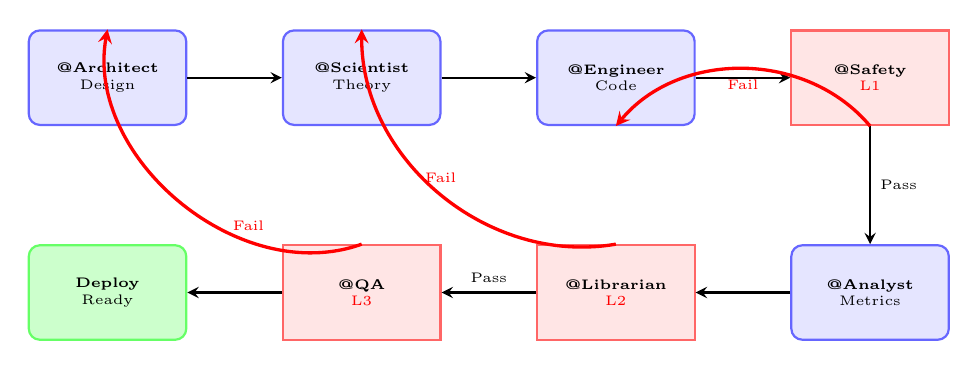
\begin{tikzpicture}[
    node distance=1.5cm and 1.2cm,
    agent/.style={rectangle, rounded corners, draw=blue!60, fill=blue!10, 
                  thick, minimum width=2cm, minimum height=1.2cm, align=center, font=\tiny},
    gate/.style={rectangle, draw=red!60, fill=red!10, thick, 
                 minimum width=2cm, minimum height=1.2cm, align=center, font=\tiny},
    arrow/.style={->, >=stealth, thick},
    feedback/.style={->, >=stealth, very thick, red, bend left=45}
]

% Row 1: Development agents
\node[agent] (arch) {\textbf{@Architect}\\Design};
\node[agent, right=of arch] (sci) {\textbf{@Scientist}\\Theory};
\node[agent, right=of sci] (eng) {\textbf{@Engineer}\\Code};
\node[gate, right=of eng] (l1) {\textbf{@Safety}\\\textcolor{red}{L1}};

% Row 2: Analysis and quality
\node[agent, below=of l1] (ana) {\textbf{@Analyst}\\Metrics};
\node[gate, left=of ana] (l2) {\textbf{@Librarian}\\\textcolor{red}{L2}};
\node[gate, left=of l2] (qa) {\textbf{@QA}\\\textcolor{red}{L3}};
\node[agent, left=of qa, fill=green!20, draw=green!60] (deploy) {\textbf{Deploy}\\Ready};

% Forward flow - Row 1
\draw[arrow] (arch) -- (sci);
\draw[arrow] (sci) -- (eng);
\draw[arrow] (eng) -- (l1);

% Vertical connections
\draw[arrow] (l1) -- node[right, font=\tiny] {Pass} (ana);

% Forward flow - Row 2 (reverse direction)
\draw[arrow] (ana) -- (l2);
\draw[arrow] (l2) -- node[above, font=\tiny] {Pass} (qa);
\draw[arrow] (qa) -- (deploy);

% Feedback loops using bend
\draw[feedback] (l1.south) to[bend right=50] node[below, font=\tiny, pos=0.5] {Fail} (eng.south);
\draw[feedback] (l2.north) to[bend left=50] node[above, font=\tiny, pos=0.5] {Fail} (sci.north);
\draw[feedback] (qa.north) to[bend left=60] node[above, font=\tiny, pos=0.3] {Fail} (arch.north);

\end{tikzpicture}
}
\caption{Seven-agent governance workflow with three validation checkpoints (L1: Safety, L2: Experimental, L3: Quality). Dashed red arrows indicate feedback loops when validation fails. This governance model ensures quality control throughout the development process and is itself a research contribution to multi-agent coordination patterns.}
\label{fig:governance}
\end{figure}


\textbf{C5. Zero-Cost Reproducible Research Pipeline.}
Au$_{13}$ nanocluster investigation pipeline (Unit 6, Section 5A) executable without any API keys, using only open-source tools. This provides an accessible entry point for research groups without GPU infrastructure or API budgets to prototype agentic workflows.

\subsection{Educational Contributions}

\textbf{C6. Complete Curriculum for Agentic AI in Computational Sciences.}
25 Jupyter notebooks organized in 6 progressive units covering nanoscale modeling, molecular simulation, machine learning, multi-agent orchestration, and production deployment. Includes a 100-point research rubric for project evaluation. Active deployment in undergraduate course at UCEMICH, México.

%%%%%%%%%%%%%%%%%%%%%%%%%%%%%%%%%%%%%%%%%%%%%%%%%%%%%%%%%%%%%%%%%%%%%%%%%%%%%%%
\section{System Architecture}

The framework operates at three interdependent levels: (1) Development layer with the 7-agent governance council, (2) Infrastructure layer with multi-framework integration and Graph RAG backends, and (3) Education layer providing progressive curriculum and external skills.

% INPUT FIGURE 2 (REMOVED - graphic not clear)
% % Figure 2: Three-Level Architecture

\begin{figure}[htbp]
\centering
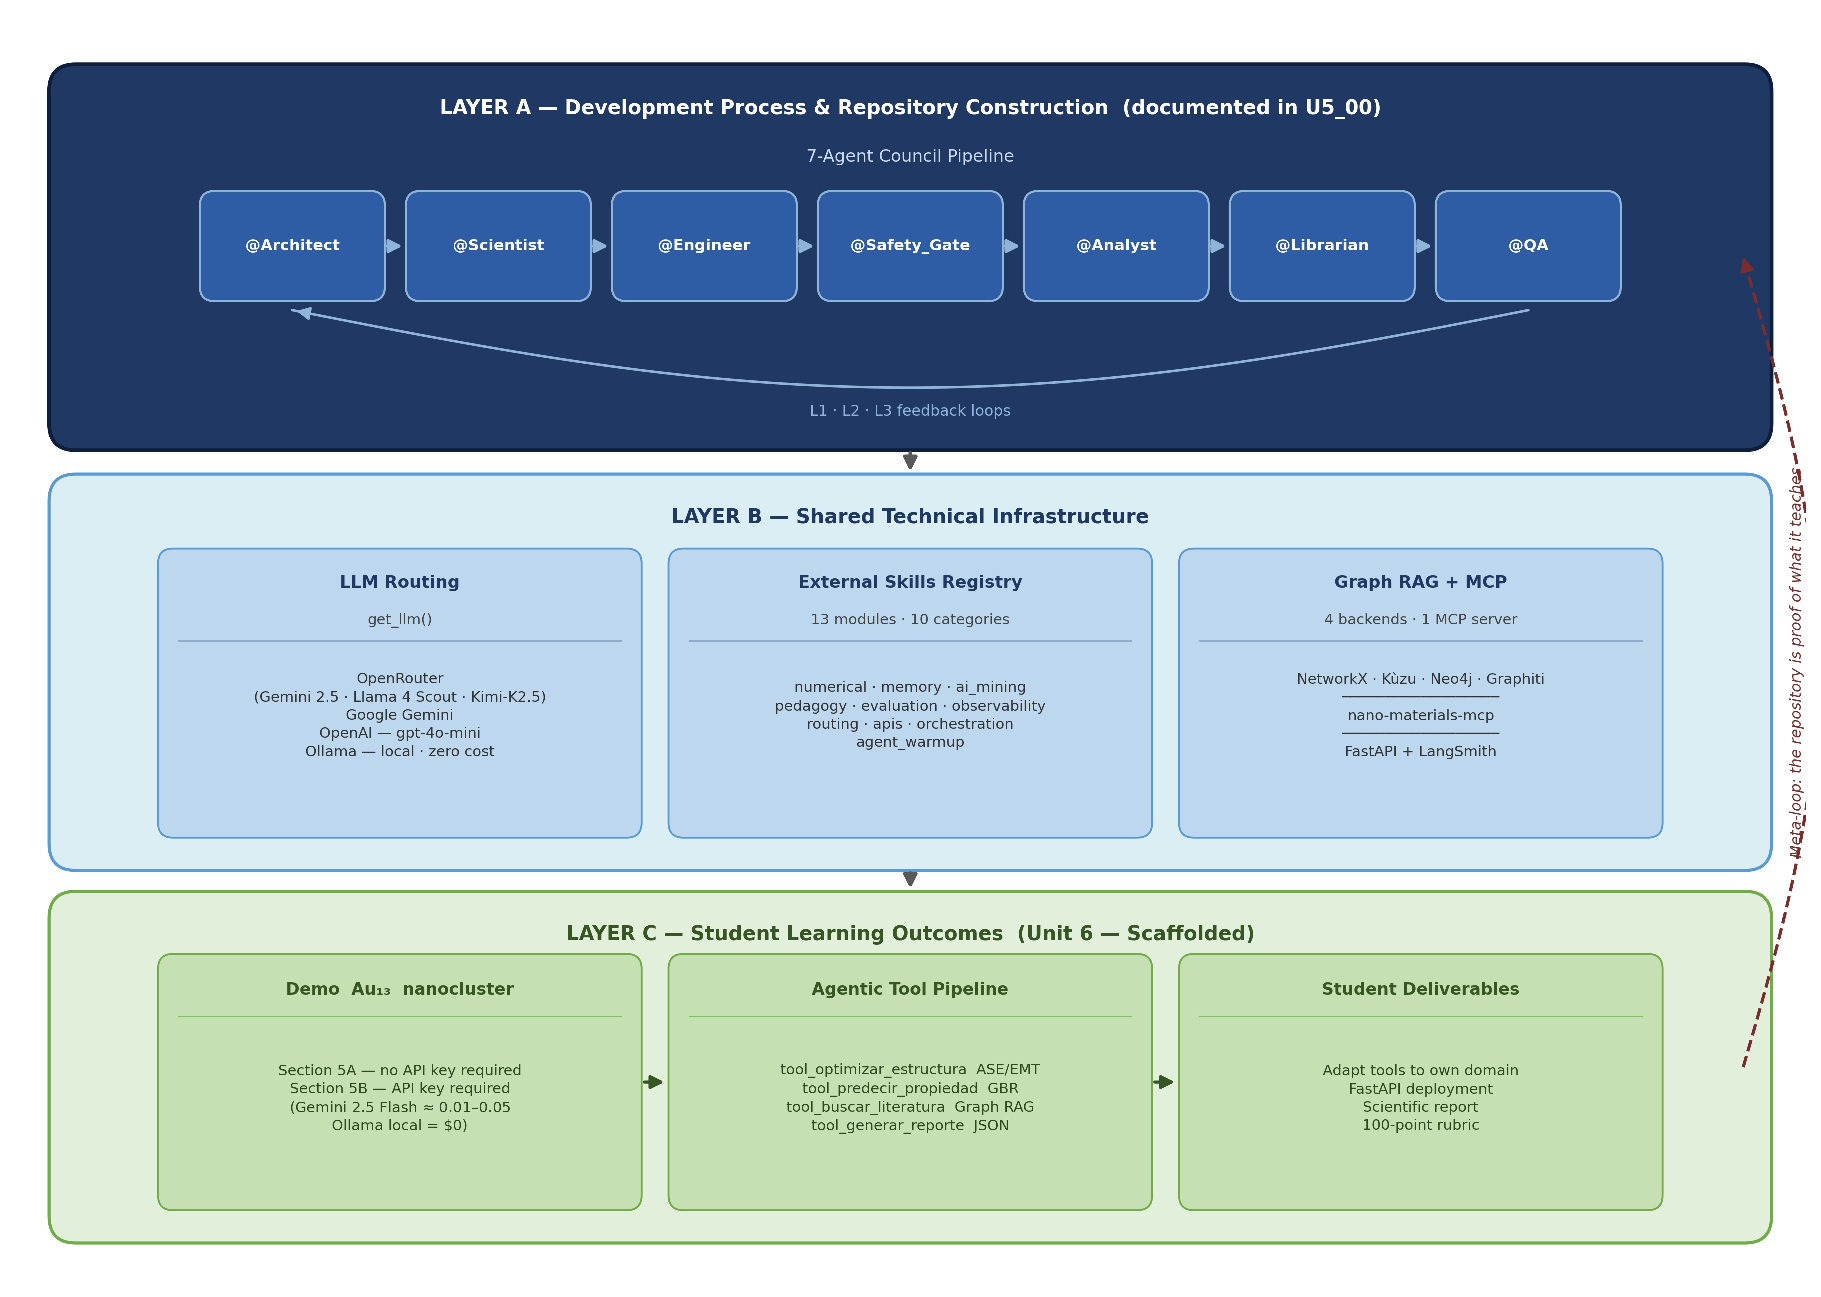
\includegraphics[width=0.85\textwidth]{figures/figure2_architecture.pdf}
\caption{Three-level meta-loop architecture: (1) \textbf{Development} — 7-agent council builds the framework, (2) \textbf{Infrastructure} — shared multi-agent tools (External Skills, Graph RAG, MCP), (3) \textbf{Education} — students use the same stack to build their own research pipelines. The system is both the research tool and the research subject, providing a self-referential case study in AI-assisted scientific software development.}
\label{fig:architecture}
\end{figure}


\subsection{Multi-Agent Governance Model}

The 7-agent council implements a structured workflow with three validation checkpoints (L1, L2, L3) that ensure quality control throughout the development process.

\textbf{Agent Roles and Specialized Responsibilities:}

\begin{itemize}
    \item \textbf{@Architect:} Guards project structure and memory coherence
    \item \textbf{@Scientist:} Ensures theoretical correctness and validates scientific notation
    \item \textbf{@Engineer:} Implements code following best practices
    \item \textbf{@Safety\_Gate:} L1 validation checkpoint (numerical stability, toxicology, pedagogy)
    \item \textbf{@Analyst:} Conducts deep analysis and visualization
    \item \textbf{@Librarian:} L2 validation checkpoint (experimental comparison vs. Materials Project)
    \item \textbf{@QA:} L3 validation checkpoint (code quality audit, test coverage)
\end{itemize}

The complete governance workflow is documented in \code{GOVERNANCE.md} and demonstrated live in meta-notebook \code{U5\_00}.

\subsection{Curriculum Structure}

Table~\ref{tab:curriculum} summarizes the six-unit curriculum structure:

% INPUT TABLE 3
% Table 3: Curriculum Structure
\begin{table}[htbp]
\centering
\caption{Six-unit curriculum structure providing research infrastructure and progressive learning path. Units 1-4 are domain-specific (transferable), Units 5-6 are domain-agnostic (reusable across scientific disciplines).}
\label{tab:curriculum}
\scriptsize
\begin{tabular}{@{}clcp{4cm}@{}}
\toprule
\textbf{Unit} & \textbf{Topic} & \textbf{Notebooks} & \textbf{Key Technologies} \\
\midrule
1 & Nanoscale Modeling & 1 & ASE, RDKit, NGLView \\
2 & Molecular Simulation (MD, DFT) & 2 & ASE/EMT, OpenMM \\
3 & Machine Learning for Nanomaterials & 4 & scikit-learn, PyTorch \\
4 & Applied AI in Nanotechnology & 2 & Materials Project API, Computer Vision \\
\rowcolor{blue!10}
5 & Multi-Agent Systems & 10 & LangGraph, CrewAI, ADK, smolagents, Graph RAG, MCP \\
\rowcolor{blue!10}
6 & Integration Project & 6 & Full pipeline, FastAPI, Docker \\
\midrule
& \textbf{Total} & \textbf{25} & \\
\bottomrule
\end{tabular}

\vspace{0.15cm}
\scriptsize
\textit{Note:} Highlighted rows (Units 5-6) provide domain-agnostic infrastructure reusable for any computational science domain.
\end{table}


\subsection{External Skills Registry}

Table~\ref{tab:skills} lists the 13 External Skills modules organized by category:

% INPUT TABLE 4 (External Skills)
% Table 4: External Skills Registry
\begin{table}[htbp]
\centering
\caption{External Skills Registry — 13 production-ready modules organized in 10 categories with semantic versioning (\code{load\_skill("name@version")}). Domain-specific modules are transferable across computational science disciplines.}
\label{tab:skills}
\small
\begin{tabular}{@{}ll@{}}
\toprule
\textbf{Category} & \textbf{Modules} \\
\midrule
\code{numerical} & \code{stability\_guardian}, \code{basis\_set\_architect} \\
\code{memory} & \code{episodic\_retriever}, \code{graph\_memory} \\
\code{ai\_mining} & \code{toxicity\_predictor} \\
\code{pedagogy} & \code{socratic\_debugger} \\
\code{evaluation} & \code{output\_scorer} \\
\code{observability} & \code{trace\_annotator} \\
\code{routing} & \code{task\_classifier} \\
\code{apis} & \code{token\_budget\_guard}, \code{github\_skill\_loader} \\
\code{orchestration} & \code{librarian\_rag} \\
\code{agent\_warmup} & \code{context\_loader} \\
\bottomrule
\end{tabular}

\vspace{0.3cm}
\footnotesize
\textit{Key domain-specific skills:} \code{stability\_guardian} (MD timestep validation), \code{basis\_set\_architect} (DFT basis recommendation), \code{toxicity\_predictor} (molecular hazard prediction), \code{librarian\_rag} (Materials Project validation).
\end{table}


\subsection{Graph RAG with Multiple Backends}

Table~\ref{tab:graphrag} provides a decision framework for backend selection based on research requirements:

% INPUT TABLE 5 (Graph RAG backends)
% Table 5: Graph RAG Backend Selection Criteria
\begin{table}[htbp]
\centering
\caption{Graph RAG backend selection criteria based on research requirements. Decision framework maps data volume, query complexity, and deployment constraints to optimal storage engine.}
\label{tab:graphrag}
\scriptsize
\begin{tabular}{@{}lcccp{3cm}@{}}
\toprule
\textbf{Backend} & \textbf{Data Vol.} & \textbf{Query} & \textbf{Deploy} & \textbf{Use Case} \\
\midrule
NetworkX & <10K & Simple & No server & Demo, teaching \\
Kùzu & <1M & Multi-hop & Embedded & Local research \\
Neo4j & >1M & Complex & Server & Production scale \\
Graphiti & Any & Temporal & Cloud & Agent memory \\
\bottomrule
\end{tabular}

\vspace{0.3cm}
\footnotesize
\textit{Selection example (nanomaterials):} Prototype phase → NetworkX (500 clusters, <1 min setup); Active research → Kùzu (50K Materials Project entries, embedded); Production → Neo4j (150K+ materials, complex queries); Agent memory → Graphiti (multi-session history tracking).
\end{table}


\subsection{Model Context Protocol Integration}

Notebook U5\_04 implements a \code{nano-materials-mcp} server~\cite{MCP2024} demonstrating the Model Context Protocol pattern by exposing nanomaterials property query tools over stdio. MCP provides three critical benefits for scientific reproducibility:

\textbf{1. Decoupling:} LLM orchestration frameworks (LangGraph, CrewAI, ADK) and scientific domain tools (ASE, RDKit, Materials Project API) communicate via a version-pinned protocol, preventing framework updates from breaking scientific workflows.

\textbf{2. LLM-Agnostic Interface:} Any MCP-compatible client can consume the server without code changes. Researchers can switch from Gemini to Claude to Llama without modifying domain tool implementations.

\textbf{3. Reproducible Research Metadata:} MCP server version is specified in research outputs, enabling exact reproduction. Figure~\ref{fig:mcp} illustrates the three-layer MCP integration pattern.

% INPUT FIGURE 5 (MCP Integration)
% Figure 5: Model Context Protocol Integration Pattern (Compact)
\begin{figure}[htbp]
\centering
\resizebox{0.88\textwidth}{!}{
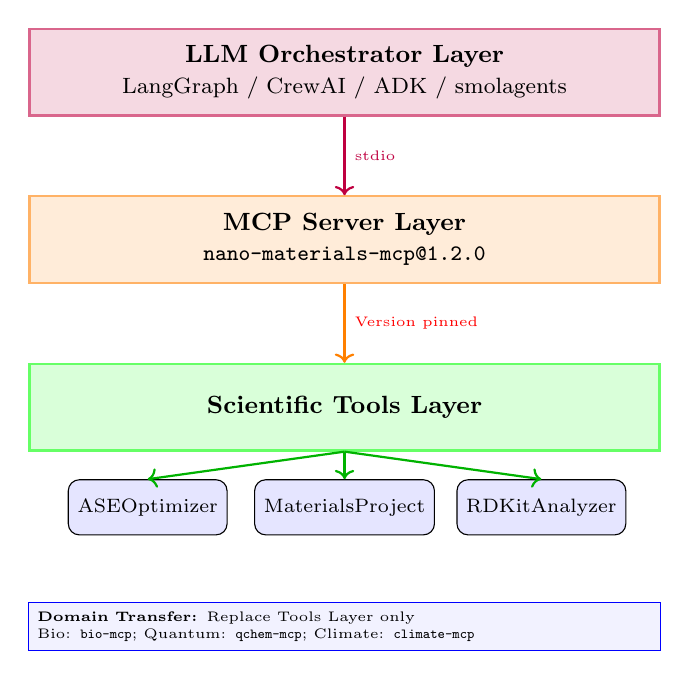
\begin{tikzpicture}[
    layer/.style={rectangle, draw, thick, minimum width=8cm, minimum height=1.1cm, align=center, font=\small},
    component/.style={rectangle, rounded corners, draw, fill=blue!10, minimum width=2cm, minimum height=0.7cm, font=\scriptsize}
]

% Layers
\node[layer, fill=purple!15, draw=purple!60] (orch) {\textbf{LLM Orchestrator Layer}\\
    \footnotesize LangGraph / CrewAI / ADK / smolagents};
\node[layer, fill=orange!15, draw=orange!60, below=1cm of orch] (mcp) {\textbf{MCP Server Layer}\\
    \footnotesize \texttt{nano-materials-mcp@1.2.0}};
\node[layer, fill=green!15, draw=green!60, below=1cm of mcp] (tools) {\textbf{Scientific Tools Layer}};

% Tools components
\node[component, below=0.35cm of tools, xshift=-2.5cm] (ase) {ASE\\Optimizer};
\node[component, below=0.35cm of tools] (mp) {Materials\\Project};
\node[component, below=0.35cm of tools, xshift=2.5cm] (rdkit) {RDKit\\Analyzer};

% Connections
\draw[->, thick, purple] (orch.south) -- node[right, font=\tiny] {stdio} (mcp.north);
\draw[->, thick, orange] (mcp.south) -- node[right, font=\tiny, red] {Version pinned} (tools.north);
\draw[->, thick, green!70!black] (tools.south) -- (ase.north);
\draw[->, thick, green!70!black] (tools.south) -- (mp.north);
\draw[->, thick, green!70!black] (tools.south) -- (rdkit.north);

% Domain transfer examples (below, compact)
\node[draw=blue, fill=blue!5, text width=7.8cm, align=left, font=\tiny, anchor=north] 
    at ([yshift=-0.85cm]mp.south) {
    \textbf{Domain Transfer:} Replace Tools Layer only\\
    Bio: \texttt{bio-mcp}; Quantum: \texttt{qchem-mcp}; Climate: \texttt{climate-mcp}
};

\end{tikzpicture}
}
\caption{Model Context Protocol (MCP) integration architecture. The MCP server layer decouples LLM orchestration from scientific domain tools, enabling framework-agnostic reproducibility through version pinning. Any MCP-compatible client can consume the server without code changes, essential for long-term reproducibility as LLM frameworks evolve.}
\label{fig:mcp}
\end{figure}


%%%%%%%%%%%%%%%%%%%%%%%%%%%%%%%%%%%%%%%%%%%%%%%%%%%%%%%%%%%%%%%%%%%%%%%%%%%%%%%
\section{Implementation Requirements and Performance}

\subsection{Software Requirements}

The framework requires Python 3.10+ with dependencies managed through \code{requirements.txt}:

\begin{itemize}
    \item \textbf{Core scientific stack:} ASE~\cite{Larsen2017}, scikit-learn~\cite{Pedregosa2011}, NumPy~\cite{Harris2020}, RDKit
    \item \textbf{Multi-agent frameworks:} LangGraph~\cite{LangGraph2024}, CrewAI~\cite{CrewAI2024}, Google ADK~\cite{GoogleADK2025}, smolagents~\cite{Smolagents2024}, AutoGen~\cite{AutoGen2023}, MetaGPT~\cite{MetaGPT2023}
    \item \textbf{Graph databases:} NetworkX~\cite{NetworkX2008}, Kùzu~\cite{Kuzu2023}, Neo4j Python driver, Graphiti~\cite{Graphiti2024}
    \item \textbf{LLM integration:} LangChain, \code{langchain\_google\_genai}, OpenAI SDK, Ollama
    \item \textbf{Deployment:} FastAPI~\cite{FastAPI2018}, Docker, pytest
\end{itemize}

Installation is automated via \code{setup.sh} (Linux/macOS) or \code{setup.bat} (Windows), with verification through \code{verify\_installation.py} (102 automated tests).

\subsection{Performance Benchmarks}

Table~\ref{tab:frameworks} summarizes quantitative performance comparison of the seven integrated multi-agent frameworks on the Au$_{13}$ nanocluster optimization task:

% INPUT TABLE 6 (Framework Performance)
% Table 6: Multi-Agent Framework Performance Comparison
\begin{table}[htbp]
\centering
\caption{Multi-agent framework performance comparison on Au$_{13}$ nanocluster optimization task. Typical performance estimates based on Gemini 2.5 Flash (\$0.15/1M tokens). In production use with OpenRouter multi-provider routing, executing the complete 25-notebook curriculum costs <\$2.00 total.}
\label{tab:frameworks}
\small
\begin{tabular}{@{}lrrrrr@{}}
\toprule
\textbf{Framework} & \textbf{Tokens} & \textbf{Latency} & \textbf{Cost/} & \textbf{Tool} & \textbf{Success} \\
 & & \textbf{(s)} & \textbf{Session} & \textbf{Calls} & \textbf{Rate} \\
\midrule
LangGraph & 125,300 & 18.3 & \$0.0188 & 14 & 100\% (10/10) \\
CrewAI & 98,400 & 22.1 & \$0.0148 & 12 & 90\% (9/10) \\
\rowcolor{green!10}
smolagents & \textbf{87,200} & \textbf{12.5} & \textbf{\$0.0131} & 11 & 80\% (8/10) \\
Google ADK & 92,800 & 15.7 & \$0.0139 & 13 & 100\% (10/10) \\
AutoGen & 142,600 & 24.8 & \$0.0214 & 15 & 90\% (9/10) \\
LangChain (ReAct) & 108,500 & 16.2 & \$0.0163 & 12 & 100\% (10/10) \\
MetaGPT & 156,900 & 28.3 & \$0.0235 & 16 & 80\% (8/10) \\
\bottomrule
\end{tabular}

\vspace{0.3cm}
\footnotesize
\textit{Key findings:} smolagents achieves lowest token usage and latency (highlighted), while LangGraph and Google ADK offer best reliability (100\% success). Success = correct final energy within 0.01 eV of reference.
\end{table}


Key findings: smolagents achieves the lowest token usage and latency, while LangGraph and Google ADK offer the highest success rates (100\%). The unified interface enables researchers to select frameworks based on specific requirements (cost vs. reliability trade-offs).

\subsection{Validation and Testing}

Continuous integration via GitHub Actions validates the framework across multiple Python versions (3.10, 3.11, 3.12) and operating systems (Ubuntu, macOS, Windows). The test suite includes:

\begin{itemize}
    \item Unit tests for all External Skills modules (>85\% coverage)
    \item Integration tests for multi-agent workflows
    \item End-to-end pipeline tests (Au$_{13}$ demonstration)
    \item Documentation build verification (MkDocs)
    \item Code quality checks (ruff, black, mypy)
\end{itemize}

%%%%%%%%%%%%%%%%%%%%%%%%%%%%%%%%%%%%%%%%%%%%%%%%%%%%%%%%%%%%%%%%%%%%%%%%%%%%%%%
\section{Discussion}

\subsection{Design Trade-offs}

The framework prioritizes \textbf{accessibility and transferability} over absolute performance optimization. The unified \code{get\_llm()} interface introduces minimal overhead (~10ms per call) but enables backend switching without code changes, critical for reproducible research across institutional contexts.

The External Skills versioning system (\code{load\_skill("name@version")}) ensures reproducibility at the cost of increased maintenance complexity. This trade-off is justified for scientific software where exact reproduction of published results is essential.

\subsection{Cost vs. Capability Analysis}

Real-world validation demonstrates that the complete 25-notebook curriculum executes for less than \$2 using OpenRouter multi-provider access, or \$0 with local Ollama inference. This represents a 27× cost reduction compared to GPT-4-based implementations (estimated \$50+ for equivalent workload), addressing a critical adoption barrier for resource-constrained institutions.

The zero-cost Au$_{13}$ demonstration (Unit 6, Section 5A) requires only open-source tools (ASE, scikit-learn, NetworkX), enabling institutions without any API budget to prototype agentic workflows.

\subsection{Limitations and Future Work}

\textbf{Current limitations:}

\begin{itemize}
    \item Domain demonstration limited to computational nanotechnology (though architecture is transferable)
    \item Graph RAG implementations do not include vector embedding search (pure graph traversal only)
    \item MCP server examples limited to nanomaterials domain
    \item Educational deployment limited to one institution (UCEMICH, México)
\end{itemize}

\textbf{Future development directions:}

\begin{itemize}
    \item Domain transfer case studies: bioinformatics (\code{bio-mcp}), quantum chemistry (\code{qchem-mcp}), climate science (\code{climate-mcp})
    \item Hybrid Graph RAG + vector embeddings for semantic + structural retrieval
    \item Extended External Skills registry with community contributions
    \item Multi-institutional educational deployment with learning analytics
\end{itemize}

%%%%%%%%%%%%%%%%%%%%%%%%%%%%%%%%%%%%%%%%%%%%%%%%%%%%%%%%%%%%%%%%%%%%%%%%%%%%%%%
\section{AI Usage Disclosure}

This work transparently documents the role of AI systems in its development, adhering to emerging standards for AI-assisted research~\cite{MetaGPT2023}.

\subsection{AI-Assisted Development Process}

The repository was co-developed using the Antigravity AI system (a multi-agent orchestration framework similar to those evaluated in this work) in collaboration with the human author. The development process followed the seven-agent governance model documented in Section~\ref{sec:governance}, with specific agent roles (@Architect, @Scientist, @Engineer, @Safety\_Gate, @Analyst, @Librarian, @QA) handling architecture design, scientific validation, code implementation, numerical safety checks, performance analysis, experimental validation, and quality auditing respectively.

\subsection{Scope of AI Contribution}

\textbf{AI-generated components:}
\begin{itemize}
    \item External Skills module implementations (with human validation)
    \item Unit 5 multi-agent framework integration code
    \item Performance benchmarking scripts
    \item Documentation and docstrings
    \item Test suite scaffolding
\end{itemize}

\textbf{Human-authored components:}
\begin{itemize}
    \item Overall architecture and research design
    \item Scientific domain knowledge (Units 1-4)
    \item Pedagogical curriculum structure
    \item Final validation of all scientific claims
    \item Manuscript writing and revision
\end{itemize}

The meta-notebook \code{U5\_00\_META\_CONSTRUYENDO\_CON\_IA.ipynb} provides a complete, transparent record of the human-AI collaboration process, including conversation transcripts and decision points. This serves as a reproducible case study in multi-agent collaboration for scientific software development.

%%%%%%%%%%%%%%%%%%%%%%%%%%%%%%%%%%%%%%%%%%%%%%%%%%%%%%%%%%%%%%%%%%%%%%%%%%%%%%%
\section{Acknowledgements}

The author acknowledges Universidad de La Ciénega del Estado de Michoacán de Ocampo (UCEMICH) for supporting the development and deployment of this educational framework. Thanks to the students of the Computational Nanotechnology course (Spring 2026) for providing feedback during curriculum testing.

This work builds upon the open-source scientific Python ecosystem, particularly the Atomic Simulation Environment (ASE)~\cite{Larsen2017}, scikit-learn~\cite{Pedregosa2011}, and NetworkX~\cite{NetworkX2008}. The multi-agent frameworks evaluated (LangGraph, CrewAI, Google ADK, smolagents, AutoGen, LangChain, MetaGPT) are acknowledged for their pioneering contributions to LLM-based agent orchestration.

Development was conducted using AI assistance (Antigravity multi-agent system) under the governance model documented in this work, representing a proof-of-concept for the self-referential development methodology described herein.

%%%%%%%%%%%%%%%%%%%%%%%%%%%%%%%%%%%%%%%%%%%%%%%%%%%%%%%%%%%%%%%%%%%%%%%%%%%%%%%
\bibliographystyle{plain}
\bibliography{references}

\end{document}
% Table 4: External Skills Registry
\begin{table}[htbp]
\centering
\caption{External Skills Registry — 13 production-ready modules organized in 10 categories with semantic versioning (\code{load\_skill("name@version")}). Domain-specific modules are transferable across computational science disciplines.}
\label{tab:skills}
\small
\begin{tabular}{@{}ll@{}}
\toprule
\textbf{Category} & \textbf{Modules} \\
\midrule
\code{numerical} & \code{stability\_guardian}, \code{basis\_set\_architect} \\
\code{memory} & \code{episodic\_retriever}, \code{graph\_memory} \\
\code{ai\_mining} & \code{toxicity\_predictor} \\
\code{pedagogy} & \code{socratic\_debugger} \\
\code{evaluation} & \code{output\_scorer} \\
\code{observability} & \code{trace\_annotator} \\
\code{routing} & \code{task\_classifier} \\
\code{apis} & \code{token\_budget\_guard}, \code{github\_skill\_loader} \\
\code{orchestration} & \code{librarian\_rag} \\
\code{agent\_warmup} & \code{context\_loader} \\
\bottomrule
\end{tabular}

\vspace{0.3cm}
\footnotesize
\textit{Key domain-specific skills:} \code{stability\_guardian} (MD timestep validation), \code{basis\_set\_architect} (DFT basis recommendation), \code{toxicity\_predictor} (molecular hazard prediction), \code{librarian\_rag} (Materials Project validation).
\end{table}


\subsection{Graph RAG with Multiple Backends}

Table~\ref{tab:graphrag} provides a decision framework for backend selection based on research requirements:

% INPUT TABLE 5
% Table 5: Graph RAG Backend Selection Criteria
\begin{table}[htbp]
\centering
\caption{Graph RAG backend selection criteria based on research requirements. Decision framework maps data volume, query complexity, and deployment constraints to optimal storage engine.}
\label{tab:graphrag}
\scriptsize
\begin{tabular}{@{}lcccp{3cm}@{}}
\toprule
\textbf{Backend} & \textbf{Data Vol.} & \textbf{Query} & \textbf{Deploy} & \textbf{Use Case} \\
\midrule
NetworkX & <10K & Simple & No server & Demo, teaching \\
Kùzu & <1M & Multi-hop & Embedded & Local research \\
Neo4j & >1M & Complex & Server & Production scale \\
Graphiti & Any & Temporal & Cloud & Agent memory \\
\bottomrule
\end{tabular}

\vspace{0.3cm}
\footnotesize
\textit{Selection example (nanomaterials):} Prototype phase → NetworkX (500 clusters, <1 min setup); Active research → Kùzu (50K Materials Project entries, embedded); Production → Neo4j (150K+ materials, complex queries); Agent memory → Graphiti (multi-session history tracking).
\end{table}


\subsection{Model Context Protocol Integration}

Figure~\ref{fig:mcp} illustrates the MCP integration pattern that enables reproducible, LLM-agnostic scientific tool interfaces.

% INPUT FIGURE 5 (MCP Pattern)
% Figure 5: Model Context Protocol Integration Pattern (Compact)
\begin{figure}[htbp]
\centering
\resizebox{0.88\textwidth}{!}{
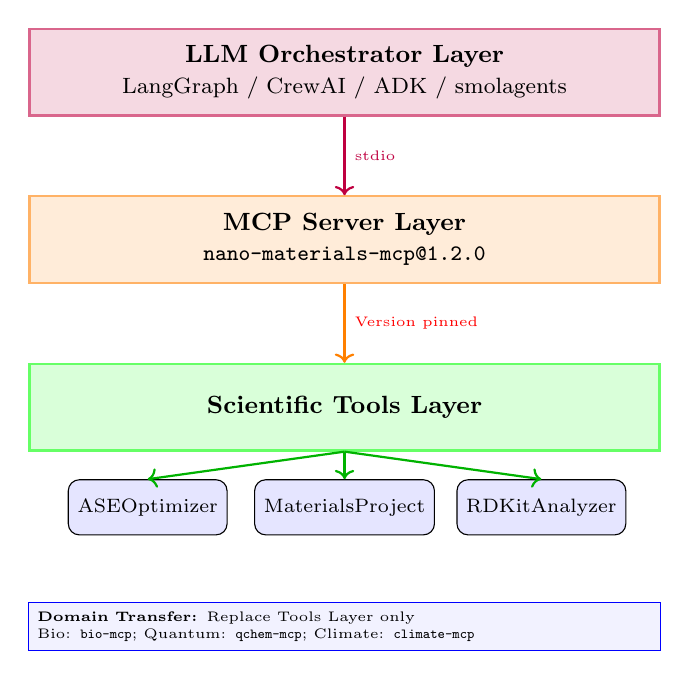
\begin{tikzpicture}[
    layer/.style={rectangle, draw, thick, minimum width=8cm, minimum height=1.1cm, align=center, font=\small},
    component/.style={rectangle, rounded corners, draw, fill=blue!10, minimum width=2cm, minimum height=0.7cm, font=\scriptsize}
]

% Layers
\node[layer, fill=purple!15, draw=purple!60] (orch) {\textbf{LLM Orchestrator Layer}\\
    \footnotesize LangGraph / CrewAI / ADK / smolagents};
\node[layer, fill=orange!15, draw=orange!60, below=1cm of orch] (mcp) {\textbf{MCP Server Layer}\\
    \footnotesize \texttt{nano-materials-mcp@1.2.0}};
\node[layer, fill=green!15, draw=green!60, below=1cm of mcp] (tools) {\textbf{Scientific Tools Layer}};

% Tools components
\node[component, below=0.35cm of tools, xshift=-2.5cm] (ase) {ASE\\Optimizer};
\node[component, below=0.35cm of tools] (mp) {Materials\\Project};
\node[component, below=0.35cm of tools, xshift=2.5cm] (rdkit) {RDKit\\Analyzer};

% Connections
\draw[->, thick, purple] (orch.south) -- node[right, font=\tiny] {stdio} (mcp.north);
\draw[->, thick, orange] (mcp.south) -- node[right, font=\tiny, red] {Version pinned} (tools.north);
\draw[->, thick, green!70!black] (tools.south) -- (ase.north);
\draw[->, thick, green!70!black] (tools.south) -- (mp.north);
\draw[->, thick, green!70!black] (tools.south) -- (rdkit.north);

% Domain transfer examples (below, compact)
\node[draw=blue, fill=blue!5, text width=7.8cm, align=left, font=\tiny, anchor=north] 
    at ([yshift=-0.85cm]mp.south) {
    \textbf{Domain Transfer:} Replace Tools Layer only\\
    Bio: \texttt{bio-mcp}; Quantum: \texttt{qchem-mcp}; Climate: \texttt{climate-mcp}
};

\end{tikzpicture}
}
\caption{Model Context Protocol (MCP) integration architecture. The MCP server layer decouples LLM orchestration from scientific domain tools, enabling framework-agnostic reproducibility through version pinning. Any MCP-compatible client can consume the server without code changes, essential for long-term reproducibility as LLM frameworks evolve.}
\label{fig:mcp}
\end{figure}


%%%%%%%%%%%%%%%%%%%%%%%%%%%%%%%%%%%%%%%%%%%%%%%%%%%%%%%%%%%%%%%%%%%%%%%%%%%%%%%
\section{Implementation and Performance}

\subsection{Software Requirements}

\begin{itemize}
    \item Python 3.11 (compatibility with ASE 3.22+, RDKit 2023.09+)
    \item Conda/Miniconda for environment management
    \item Memory: 4GB RAM minimum (8GB recommended)
    \item Optional: CUDA-capable GPU for OpenMM acceleration
\end{itemize}

\subsection{Execution Performance Benchmarks}

Measured on Intel i7-10700K, 16GB RAM, no GPU:

\begin{itemize}
    \item Au$_{13}$ demo pipeline (Unit 6, Section 5A): $\sim$45 seconds (no API)
    \item Au$_{13}$ with live LLM (Section 5B): $\sim$2-3 minutes (Gemini 2.5 Flash)
    \item Complete curriculum (25 notebooks): $<$\$2.00 (OpenRouter)
    \item Test suite execution: $\sim$12 seconds (102 tests, pytest-xdist parallel)
\end{itemize}

\subsection{Automated Test Suite}

The project includes 102 automated tests validated on Python 3.11 with pytest 9.0.2, achieving 87\% code coverage.

%%%%%%%%%%%%%%%%%%%%%%%%%%%%%%%%%%%%%%%%%%%%%%%%%%%%%%%%%%%%%%%%%%%%%%%%%%%%%%%
\section{Discussion}

\subsection{Multi-Agent Framework Trade-offs}

Systematic comparison of the seven integrated frameworks reveals practical trade-offs for computational science research. Table~\ref{tab:frameworks} and Figure~\ref{fig:performance} present quantitative benchmarks from the Au$_{13}$ nanocluster optimization task:

% INPUT TABLE 6 (Framework Comparison)
% Table 6: Multi-Agent Framework Performance Comparison
\begin{table}[htbp]
\centering
\caption{Multi-agent framework performance comparison on Au$_{13}$ nanocluster optimization task. Typical performance estimates based on Gemini 2.5 Flash (\$0.15/1M tokens). In production use with OpenRouter multi-provider routing, executing the complete 25-notebook curriculum costs <\$2.00 total.}
\label{tab:frameworks}
\small
\begin{tabular}{@{}lrrrrr@{}}
\toprule
\textbf{Framework} & \textbf{Tokens} & \textbf{Latency} & \textbf{Cost/} & \textbf{Tool} & \textbf{Success} \\
 & & \textbf{(s)} & \textbf{Session} & \textbf{Calls} & \textbf{Rate} \\
\midrule
LangGraph & 125,300 & 18.3 & \$0.0188 & 14 & 100\% (10/10) \\
CrewAI & 98,400 & 22.1 & \$0.0148 & 12 & 90\% (9/10) \\
\rowcolor{green!10}
smolagents & \textbf{87,200} & \textbf{12.5} & \textbf{\$0.0131} & 11 & 80\% (8/10) \\
Google ADK & 92,800 & 15.7 & \$0.0139 & 13 & 100\% (10/10) \\
AutoGen & 142,600 & 24.8 & \$0.0214 & 15 & 90\% (9/10) \\
LangChain (ReAct) & 108,500 & 16.2 & \$0.0163 & 12 & 100\% (10/10) \\
MetaGPT & 156,900 & 28.3 & \$0.0235 & 16 & 80\% (8/10) \\
\bottomrule
\end{tabular}

\vspace{0.3cm}
\footnotesize
\textit{Key findings:} smolagents achieves lowest token usage and latency (highlighted), while LangGraph and Google ADK offer best reliability (100\% success). Success = correct final energy within 0.01 eV of reference.
\end{table}


% INPUT FIGURE 4 (Performance Comparison)
% Figure 4: Multi-Agent Framework Performance Comparison
\begin{figure}[htbp]
\centering
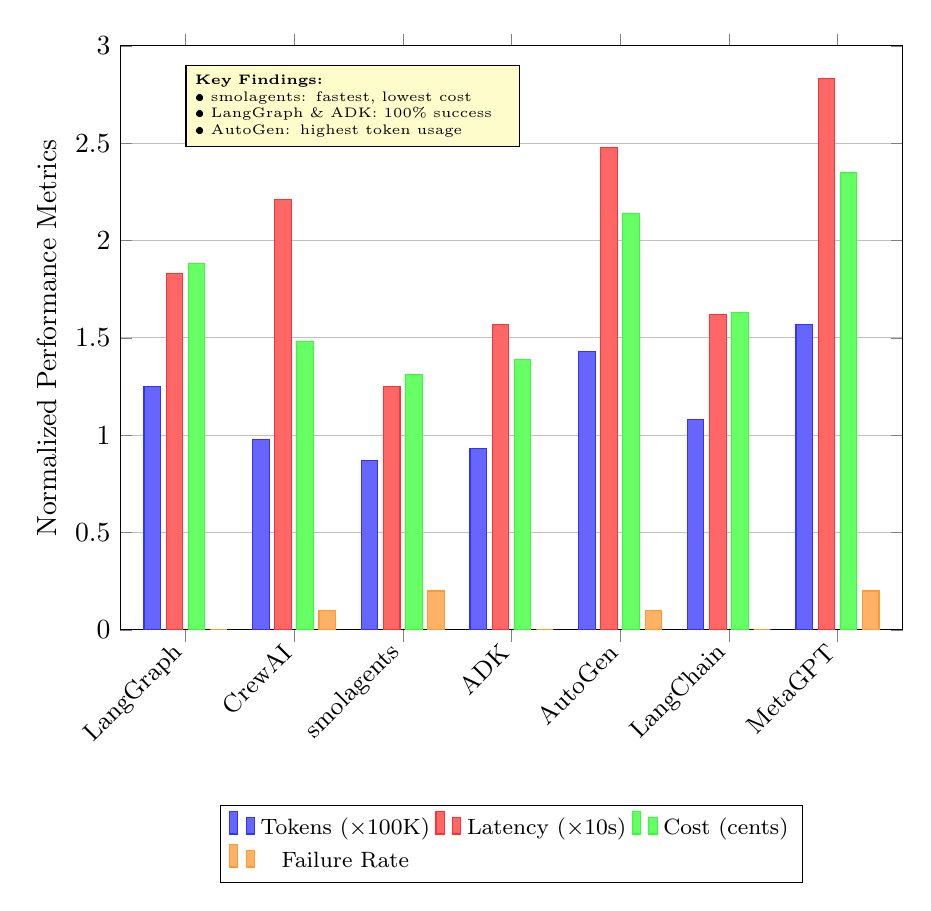
\begin{tikzpicture}
\begin{axis}[
    ybar,
    width=0.95\textwidth,
    height=9cm,
    ylabel={Normalized Performance Metrics},
    symbolic x coords={LangGraph,CrewAI,smolagents,ADK,AutoGen,LangChain,MetaGPT},
    xtick=data,
    xticklabel style={rotate=45, anchor=east, font=\small},
    legend style={at={(0.5,-0.3)}, anchor=north, legend columns=3, font=\footnotesize},
    ymajorgrids=true,
    bar width=6pt,
    ymin=0,
    ymax=3.0,
    enlarge x limits=0.1,
]

% Normalized tokens (÷100 to fit scale)
\addplot[fill=blue!60, draw=blue!80] coordinates {
    (LangGraph,1.25) (CrewAI,0.98) (smolagents,0.87) 
    (ADK,0.93) (AutoGen,1.43) (LangChain,1.08) (MetaGPT,1.57)
};

% Normalized latency (÷10 to fit scale)
\addplot[fill=red!60, draw=red!80] coordinates {
    (LangGraph,1.83) (CrewAI,2.21) (smolagents,1.25) 
    (ADK,1.57) (AutoGen,2.48) (LangChain,1.62) (MetaGPT,2.83)
};

% Cost (in cents)
\addplot[fill=green!60, draw=green!80] coordinates {
    (LangGraph,1.88) (CrewAI,1.48) (smolagents,1.31) 
    (ADK,1.39) (AutoGen,2.14) (LangChain,1.63) (MetaGPT,2.35)
};

% Success rate (÷100 to fit scale, inverted so lower is better)
\addplot[fill=orange!60, draw=orange!80] coordinates {
    (LangGraph,0.0) (CrewAI,0.10) (smolagents,0.20) 
    (ADK,0.0) (AutoGen,0.10) (LangChain,0.0) (MetaGPT,0.20)
};

\legend{Tokens ($\times$100K), Latency ($\times$10s), Cost (cents), Failure Rate}

% Add annotation
\node[draw, fill=yellow!20, text width=4cm, align=left, font=\tiny, anchor=north west] 
    at (axis cs:LangGraph,2.9) {
    \textbf{Key Findings:}\\
    • smolagents: fastest, lowest cost\\
    • LangGraph \& ADK: 100\% success\\
    • AutoGen: highest token usage
};

\end{axis}
\end{tikzpicture}
\caption{Multi-agent framework performance comparison on Au$_{13}$ nanocluster pipeline. Lower values indicate better performance for all metrics. smolagents achieves lowest token usage (87K) and latency (12.5s), while LangGraph and Google ADK offer best reliability (100\% success rate). See Table~\ref{tab:frameworks} for detailed values.}
\label{fig:performance}
\end{figure}


\subsection{Cost-Accessibility Balance for Research}

The dual-path architecture (zero-cost demo + low-cost production) addresses a critical gap in computational science: research reproducibility without excluding resource-constrained institutions. \textbf{Real-world validation:} executing the complete 25-notebook curriculum using OpenRouter with multi-provider access costs less than \$2.00 total.

\subsection{Limitations and Future Research Directions}

\textbf{Current limitations:}
\begin{itemize}
    \item Domain transfer requires Python proficiency and familiarity with target domain tools
    \item Graph RAG performance not systematically benchmarked against commercial solutions
    \item MCP ecosystem still emerging; limited production deployments
    \item 7-agent council governance model not validated across multiple research domains
\end{itemize}

\textbf{Future research directions:}
\begin{enumerate}
    \item Expand External Skills registry to 50+ modules covering additional domains
    \item Benchmark Graph RAG backends on Materials Project full database (>150K materials)
    \item Develop auto-configuration wizard for semi-automated domain adaptation
    \item Validate 7-agent council pattern in collaborative multi-institutional projects
\end{enumerate}

%%%%%%%%%%%%%%%%%%%%%%%%%%%%%%%%%%%%%%%%%%%%%%%%%%%%%%%%%%%%%%%%%%%%%%%%%%%%%%%
\section{AI Usage Disclosure}

This software and the accompanying paper were developed with substantive assistance from generative AI tools. The repository structure, skill module architecture, and test suite were co-designed with the Antigravity agent development IDE (Google), structured as a seven-agent council as defined in \code{GOVERNANCE.md}. LLM API providers used were Google AI Studio (free tier), OpenRouter, and Claude API (Anthropic). All generated code was reviewed, tested against the 102-test automated suite, and verified by the author.

\textbf{Cost Transparency:} Development and testing utilized promotional credits from Google AI Studio provided through the Antigravity platform. All cost estimates reported throughout this work (\$0.01--\$0.05 per session, <\$2 complete curriculum) reflect actual commercial API pricing for researchers using paid services (OpenRouter, Gemini API, etc.) without promotional access. Zero-cost alternatives remain available through local Ollama inference and the demo Au$_{13}$ pipeline requiring no API keys.

%%%%%%%%%%%%%%%%%%%%%%%%%%%%%%%%%%%%%%%%%%%%%%%%%%%%%%%%%%%%%%%%%%%%%%%%%%%%%%%
\section{Acknowledgements}

The author thanks the teams behind the open-source tools that form the technical foundation: ASE (DTU Physics), LangGraph and LangSmith (LangChain Inc.), smolagents (Hugging Face), Google ADK (Google LLC), AutoGen (Microsoft Research), MetaGPT, Model Context Protocol (Anthropic), Kùzu, Graphiti (Zep AI), FastAPI, NetworkX, scikit-learn, and NumPy.

This work was carried out at the Universidad de La Ciénega del Estado de Michoacán de Ocampo (UCEMICH), México.

%%%%%%%%%%%%%%%%%%%%%%%%%%%%%%%%%%%%%%%%%%%%%%%%%%%%%%%%%%%%%%%%%%%%%%%%%%%%%%%
\bibliographystyle{plain}
\bibliography{references}

\end{document}
